% Comparing two methods for the modeling of water
\subsection{Comparaison de deux méthodes pour la molécule d'eau} \label{sec:h2o}

Puisque l'eau joue un rôle important dans le système que nous étudions, nous voulons explorer plusieurs approches pour la modélisation de la molécule d'eau :
\begin{itemize}
    \item le modèle \emph{Extended Simple Point Charge} (abrégé \spce{})\cite{pullman_interaction_1981}\cite{berendsen_missing_1987}
    \item le potentiel réactif \reaxff{} (présenté à la \autoref{sec:reaxff})
\end{itemize}

Nous faisons d'abord une brève comparaison des fonctionnements théoriques des deux méthodes, puis mettons en place des simulations d'un même système avec ces deux approches, et finalement comparons leurs résultats.

\textbf{Comparaison des fonctionnements}\\
Alors que le potentiel \reaxff{} est réactif et se base sur les ordres de liaison (voir \autoref{sec:reaxff}), le modèle \spce{} est rigide et les interactions intermoléculaires ne considèrent que les atomes d'oxygène avec un potentiel de Lennard--Jones.

\begin{table}[h!]
    \centering
    \begin{tabular}{l || c | c}
        \hline
        Caractéristiques               & \reaxff{}         & \spce{}           \\
        \hline
        Modèle de liaisons             & Ordres de liaison & Rigide/Harmonique \\
        Modèle d'angles                & Ordres de liaison & Rigide/Harmonique \\
        Modèle de molécules            & Aucun             & Rigide            \\
        Interactions intermoléculaires & \reaxff{}         & Lennard--Jones    \\
        \hline
    \end{tabular}
    \caption{Comparaison des fonctionnements des modèles}
    \label{tab:comparaison_modeles}
\end{table}

De fait, \reaxff{} est un potentiel objectivement plus flexible que le modèle \spce{} mais implique une charge de calcul beaucoup plus grande.

Par ailleurs, puisque le modèle \spce{} fait appel à des molécules/liaisons/angles rigides, son utilisation avec \lammps{} nécessite l'utilisation d'un format de données de configuration initiale plus complet que \reaxff{}. La conversion des données dans ce format est détaillée à l'\autoref{apdx:conversion_spce}.

\textbf{Mise en place des simulations}\\
Pour faciliter la comparaison des résultats obtenus par simulations aux résultats expérimentaux, les conditions de simulations sont : $T = \qty{300}{\kelvin}, P = \qty{1}{\atm}$, et les simulations suivent le déroulement présenté à la \autoref{sec:deroulement_simulations}. Les différentes quantités thermodynamiques relevées au cours de ces simulations sont présentées aux \autoref{fig:h2o_relaxation} et \ref{fig:h2o_main}.

\begin{figure}[h!]
    \centering
    \begin{subfigure}{.49\textwidth}
        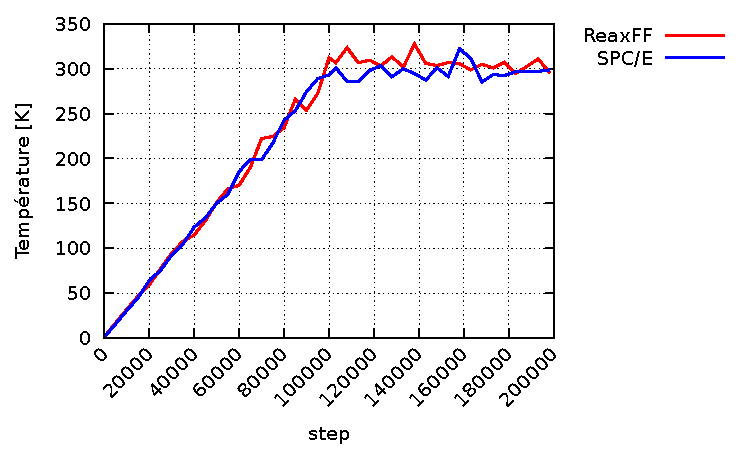
\includegraphics[width = \textwidth, draft]{h2o_relaxation_temp.pdf}
        \caption{Températures}
    \end{subfigure}%
    ~
    \begin{subfigure}{.49\textwidth}
        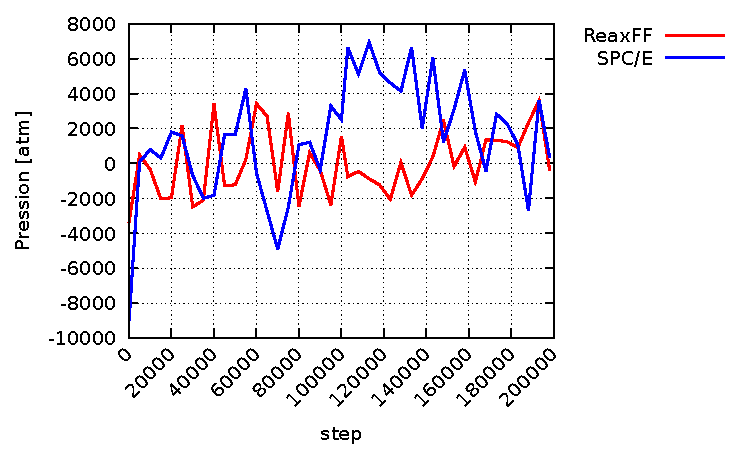
\includegraphics[width = \textwidth, draft]{h2o_relaxation_press.pdf}
        \caption{Pressions}
    \end{subfigure}
    \begin{subfigure}{.49\textwidth}
        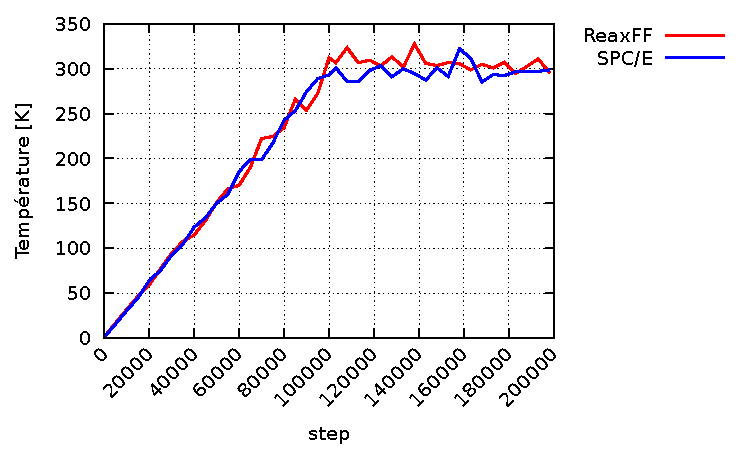
\includegraphics[width = \textwidth, draft]{h2o_relaxation_temp.pdf}
        \caption{Densités}
    \end{subfigure}
    \caption{Quantités thermodyanmiques lors de la relaxation}
    \label{fig:h2o_relaxation}
\end{figure}

\begin{figure}[h!]
    \centering
    \begin{subfigure}{.49\textwidth}
        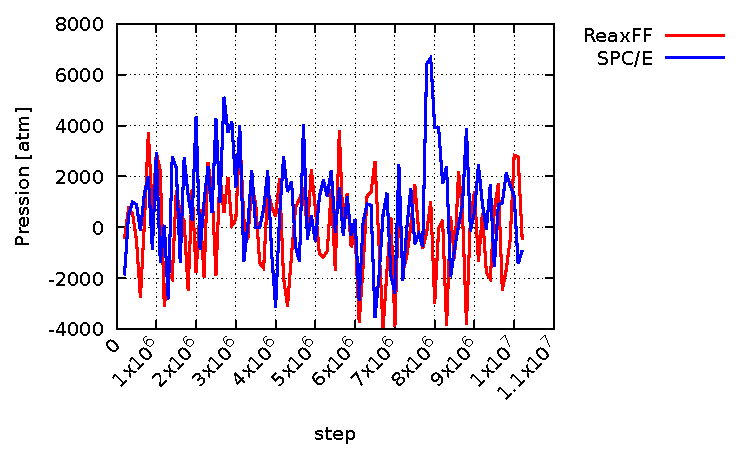
\includegraphics[width = \textwidth, draft]{h2o_main_press.pdf}
        \caption{Pressions}
    \end{subfigure}%
    ~
    \begin{subfigure}{.49\textwidth}
        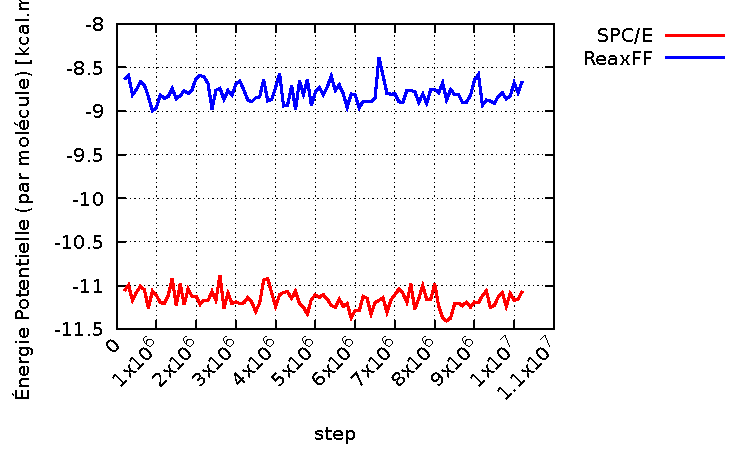
\includegraphics[width = \textwidth, draft]{h2o_main_epot.pdf}
        \caption{Énergies potentielles totales}
    \end{subfigure}
    \caption{Quantités thermodynamiques lors de la simulation}
    \label{fig:h2o_main}
\end{figure}

\textbf{Proriétés comparées}\\
Pour cette étude, nous comparons les propriétés structurales et de diffusion des deux modèles avec la \emph{Radial Distribution Function} et le \emph{Mean Squared Displacement}.

En effet, pour rappel, la première des deux grandeurs nous informe sur la probabilité de trouver deux atomes à une distance donnée l'un de l'autre en comparaison à un gaz parfait :
\begin{equation}
    \boxed%
    {
        g (r) = \frac{\left\langle \rho (r) \right\rangle}{\rho} = \frac{\mathrm{d}n(r)}{4 \pi r^2 \mathrm{d}r \rho}
    }
    \label{eq:rdf}
\end{equation}
où $\rho (r)$ est la densité locale de particules, $\left\langle \cdot \right\rangle$ est la moyenne sur l'ensemble, $\mathrm{d}n(r)$ est le nombre de particules à l'intérieur de la coquille sphérique située à $r$ et d'épaisseur $\mathrm{d}r$, et $\rho$ est la densité numérique moyenne de la paire considérée.

Quant à la deuxième quantité, pour des temps sufisamment longs elle nous donne indirectement le coefficient de diffusion du système :
\begin{equation*}
    MSD(t) \equiv \left\langle \left| \vec{r}(t) - \vec{r}(t_0) \right|^2 \right\rangle = 2 d D t
\end{equation*}
où $\vec{r}$ est la position d'une particule, $\left\langle \cdot \right\rangle$ est la moyenne sur l'ensemble, $t_0$ est un temps de référence, $d$ est le nombre de dimensions du problème, $D$ est le coefficient de diffusion du système et $t$ est le temps.

Cependant, pour obtenir une meilleur précision quant au coefficient de diffusion, nous utilisons le \emph{Mean Squared Displacement} moyenné sur les décalages en temps :
\begin{equation}
    \boxed%
    {
        \overline{MSD} (\tau) = \frac{1}{N_{\tau}} \sum_{i = 0}^{N_{\tau}} \left\langle \left| \vec{r}(\tau) - \vec{r}(t_0) \right|^2 \right\rangle  = 2 d D t
    }
\end{equation}
où $\tau$ est un décalage de configurations, et $N_{\tau}$ le nombre de configurations pouvant être décalées de $\tau$ dans la trajectoire. $\overline{MSD}$ est donc, pour chaque décalage de configurations, une moyenne sur l'ensemble de la trajectoire.

\textbf{Résultats obtenus}\\
LES RÉSULTATS !!

\begin{figure}[h!]
    \centering
    \begin{subfigure}{.49\textwidth}
        \includegraphics[width = \textwidth, draft]{h2o_rdf.pdf}
        \caption{Comparaison des \emph{Radial Distribution Function}s}
        \label{fig:h2o_rdf}
    \end{subfigure}
    \begin{subfigure}{.49\textwidth}
        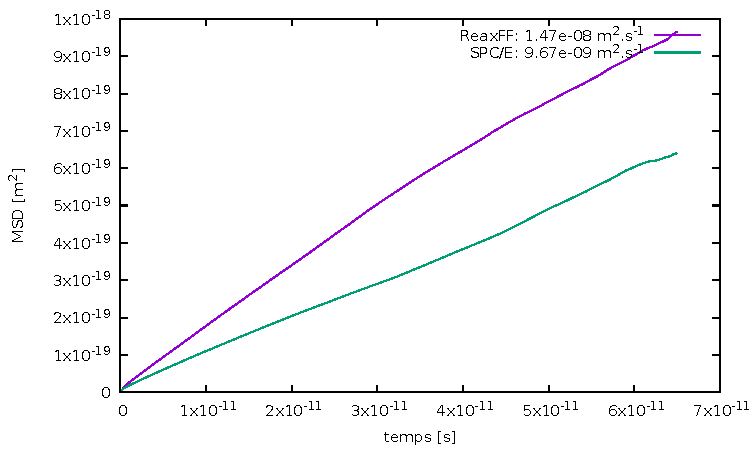
\includegraphics[width = \textwidth, draft]{h2o_msd.pdf}
        \caption{Comparaison des \emph{Mean Squared Displacement}s}
        \label{fig:h2o:msd}
    \end{subfigure}
    \caption{Comparaison des résultats obtenus}
    \label{fig:h2o_comparaison_resultats}
\end{figure}
